\section{Monadic second-order logics and modal $\mu$-calculi}
\label{s:mso-mu}

In this section we introduce the main logics of our narrative, i.e., the weak 
and noetherian versions of monadic second-order logic on the one hand, and the 
continuous and noetherian fragments of the modal $\mu$-calculus on the other.
We also briefly discuss some model-theoretic properties and results related to 
these logics.

\subsection{Monadic second-order logics}
\label{sec:prel-so}

Three variations of monadic second-order logic feature in our work:
\emph{standard}, \emph{weak}, and \emph{noetherian} monadic second-order 
logic, and for each of these three variations, we consider a one-sorted and 
a two-sorted version.
As we will see later, the one-sorted version fits better in the 
automata-theoretic framework, whereas it is more convenient to use the 
two-sorted approach when translating $\mu$-calculi to second order languages.
In both the one-sorted and the two-sorted version, the syntax of the three 
languages is the same, the difference lying in the semantics, more specificaly,
in the type of subsets over which the second-order quantifiers range.
In the case of standard and weak monadic second-order logic, these quantifiers 
range over all, respectively, all finite subsets of the model.
In the case of \nmso we need the concept of a \emph{noetherian} subset of an LTS.

\begin{definition}
\label{d:bundle1}
Let $\bbS = \tup{T,R,\tscolors, s_I}$ be an LTS, and let $B$ be a set of finite
paths that all share the same starting point $s$; we call $B$ a \emph{bundle 
rooted at} $s$, or simply an $s$-\emph{bundle}, if $B$ does not contain an
infinite ascending chain $\pi_{0} \sqsubset \pi_{1} \sqsubset 
\cdots$, where $\sqsubset$ denotes the (strict) initial-segment relation on 
paths.
A \emph{bundle} is simply an $s$-bundle for some $s \in T$.
Finally, a subset $X$ of $T$ is called \emph{noetherian} if there is a bundle 
$B$ such that each $t \in X$ lies on some path in $B$.
\end{definition}

\begin{example} 
\label{ex:noeth}
Let $\bbS = \tup{T,R,\tscolors, s_I}$ be a labelled transition system.
\begin{enumerate} 
\item
Since the empty bundle is a bundle, the empty set is a noetherian set in $\bbS$.
\item
In case $\bbS$ is a conversely well-founded tree, the set of all paths emanating
from $s_{I}$ is a bundle, and therefore \emph{every} subset of $T$ is 
noetherian.
\item
More generally, if $\bbS$ is an arbitrary tree, its noetherian subsets coincide
with those that are included in a well-founded subtree of $\bbS$.
In case $\bbS$ is finitely branching, every well-founded subtree is finite; as a  
consequence, every noetherian subset is finite.
\item
Let $s$ be some arbitrary node in $\bbS$, and suppose that the points $s_{1},
\ldots,s_{n}$ are all reachable from $s$ (i.e., belong to the set 
$R^{*}[s]$).
Then for each $i$ we may fix a (finite) path $\pi_{i}$ from $s$ to $s_{i}$.
Clearly these paths, taken together, provide a bundle, and so the set $\{ s_{1},
\ldots,s_{n} \}$ is noetherian.
\item
This means in particular that every singleton is noetherian.
Furthermore, if $\bbS$ is finite, and every point in $\bbS$ is reachable from 
$s_{I}$, then every subset of $T$ is noetherian.
\item
\label{ex-it:n}
Similarly, every finite subset of a tree is noetherian.
Hence, on finitely branching trees, the noetherian sets coincide with the finite
ones.
\end{enumerate}
\end{example}

\subsubsection*{One-sorted monadic second-order logics}
%
\begin{definition}\label{def:mso}
The formulas of the \emph{(one-sorted) monadic second-order language} are
defined by the following grammar:
%
\begin{eqnarray*}\label{EQ_mso}
  \phi \isbnf  \here{p} \mid p \inc q \mid R(p,q) \mid \lnot\phi 
     \mid \phi\lor\phi \mid \exists p.\phi,
\end{eqnarray*}
where $p$ and $q$ are letters from $\Prop$.
We  adopt the standard convention that no proposition letter is both free and
bound in $\phi$.
\end{definition}


As mentioned, the three logics $\smso$, $\wmso$ and $\nmso$ are distinguished by
their semantics. 
Let  $\bbS = \tup{T,R,\tscolors, s_I}$ be an LTS.
The interpretation of the atomic formulas is fixed:
\begin{align*}
    \bbS \models \here{p} & \quad\text{ iff }\quad  \tsval(p) = \{s_I\} 
\\ \bbS \models p \inc q & \quad\text{ iff }\quad  \tsval(p) \subseteq \tsval(q)
\\ \bbS \models R(p,q) & \quad\text{ iff }\quad  
  \text{for every $s\in \tsval(p)$ there exists $t\in \tsval(q)$ such that $sRt$.} 
\end{align*}
Furthermore, the interpretation of the boolean connectives is standard.
The interpretation of the existential quantifier is where the logics diverge:

\begin{align*}
\bbS \models\ \exists p. \phi  & \quad\text{ iff }\quad  \bbS[p \mapsto X] \models \phi \,
\left.\begin{cases}
   \text{for some }                   & (\smso)
\\ \text{for some \emph{finite} }     & (\wmso) 
\\ \text{for some \emph{noetherian} } & (\nmso)
\end{cases}\right\}\,
 X \subseteq T.
\end{align*}

Observe that for a given monadic second-order formula $\phi$, the classes 
$\Mod_{\smso}(\phi)$, $\Mod_{\wmso}(\phi)$ and $\Mod_{\nmso}(\phi)$ will 
generally be different.

\subsubsection*{Two-sorted monadic second-order logics}
The reader may have expected to see the following more standard language for
second-order logic.
\begin{definition}
\label{def:2mso}
Given a set $\fovar$ of individual (first-order) variables, we define the 
formulas of the \emph{two-sorted monadic second-order language} by the following
grammar:
\[
\phi \isbnf  p(x)
\mid R(x,y)
\mid x \foeq y
\mid \neg \phi
\mid \phi \lor \phi
\mid \exists x.\phi
\mid \exists p.\phi
\]
where $p \in \Prop$, $x,y \in \fovar$ and $\foeq$ is the symbol for equality.   
\end{definition}

Formulas are interpreted over an LTS $\bbS = \tup{T,R,\tscolors, s_I}$ with a
variable assignment $g: \fovar \to T$, and the semantics of the language is
completely standard. 
Depending on whether second-order quantification ranges over all subsets, over 
finite subsets or over noetherian subsets, we obtain the three two-sorted 
variations denoted respectively as $2\smso$, $2\wmso$ and $2\nmso$.

\subsubsection*{Equivalence of one-sorted and two-sorted MSO}
In each variation, the one-sorted and the two-sorted versions can be proved to
be equivalent, but there is a subtlety due to the fact that our models have a 
distinguished state.
In the one-sorted language, we use the downarrow $\here$ to access this
distinguished state; in the two-sorted approach, we will use a \emph{fixed}
variable $v$ to refer to the distinguished state, and given a formula 
$\phi(v)$ of which $v$ is the only free individual variable, we write 
$\bbS \models \phi[s_{I}]$ rather than $\bbS[v \mapsto s_{I}] \models \phi$.
As a consequence, the proper counterpart of the one-sorted language $\smso$ is
the set $2\smso(v)$ of those $2\smso$-formulas that have precisely $v$ 
as their unique free variable.

More in particular, with $L \in \{\smso, \wmso, \nmso\}$, we say that $\phi \in
L$ is \emph{equivalent to} $\psi(v) \in L(v)$ if
\[
\bbS \models \phi \text{ iff } \bbS \models \psi[s_{I}]
\]
for every model $\bbS = \tup{T,R,\tscolors, s_I}$.
We can now state the equivalence between the two approaches to 
monadic second-order logic as follows.

\begin{proposition}
\label{p:msovs2mso}
Let $L \in \{\smso, \wmso, \nmso\}$ be a monadic second-order logic.
\begin{enumerate}
\item
There is an effective construction transforming a formula $\phi \in L$ into
an equivalent formula $\phi^{t} \in 2L(v)$.
\item
There is an effective construction transforming a formula $\psi \in 2L(v)$ into
an equivalent formula $\psi^{o} \in L$.
\end{enumerate}
\end{proposition}

\begin{proof}
Since it is completely straightforward to define a translation $(\cdot)^{t}$ as 
required for part (1) of Proposition~\ref{p:msovs2mso}, we only discuss the proof 
of part (2). 
The key observation here is that a single-sorted language can interpret the 
corresponding two-sorted language by encoding every individual variable $x \in 
\fovar$ as a set variable $p_x$ denoting a singleton, and that it is easy to 
write down a formula stating that a variable indeed is interpreted by a 
singleton.
As a consequence, where $2\yvlang(\pprop,\mathsf{X})$ denotes the set of
$2L$-formulas with free second-order variables in $\pprop$ and free first-order
variables in $\mathsf{X}$, it is not hard to formulate a translation 
$(\cdot)^{m} : 2\yvlang(\pprop,\mathsf{X}) \to \yvlang(\pprop \uplus 
\{ p_{x} \mid x \in \mathsf{X} \})$
such that, for every model $\bbS$, every variable assignment $g$ and every
formula $\psi \in 2\yvlang(\Prop,\mathsf{X})$:
\[
\bbS,g \models \psi \quad\text{iff}\quad 
\bbS[p_{x} \mapsto \{g(x)\} \mid x \in \mathsf{X}] \models \psi^m.
\]
From this it is immediate that any $\psi \in 2L(v)$ satisfies
\[
\bbS \models \psi[s_{I}]
\quad\text{iff}\quad 
\bbS \models \exists p_{v} (\here{p_{v}} \land \psi^{m}),
\]
so that we may take $\psi^{o} \isdef \exists p_{v} (\here{p_{v}} \land 
\psi^{m})$.
\end{proof}

Comparing the relative expressive power of the logics $\smso$, $\wmso$ and 
$\nmso$ on finitely trees, on arbitrary trees, and on arbitrary models, we can
make the following observations.
\begin{description}
\item[Finitely branching trees] 
From Example~\ref{ex:noeth}(\ref{ex-it:n}) it follows that on this subclass of
LTS, $\nmso$ and $\wmso$ are equivalent. 
They are however both strictly included in $\smso$. 
First of all,  since being a well-founded subtree is $\smso$ definable, $\nmso$ 
(and thus $\wmso$) is included in $\smso$.
Finally, from \cite{Rab70}, we know that already on binary trees the 
$\smso$-definable property ``there is a path on which $p$ is true infinitely 
often'' is not $\wmso$ definable.  
\item[Arbitrary trees] 
For the same reason as in the case of finitely branching trees, $\nmso$ is 
strictly included in $\smso$. 
However, $\wmso$ is now incomparable with both $\nmso$  and $\smso$. 
First,  it is well known that $\wmso$ can only define properties whose 
topological complexity is Borel (see e.g. \cite{CateF11}), whereas $\nmso$ can 
also define non Borel properties, such as being well-founded. 
Second, consider the property of having a node with infinitely many successors. 
This property is clearly definable in $\wmso$, but not in $\smso$. 
This is due to the fact that on arbitrary trees every $\smso$ formula is
equivalent to a MSO-automata and that every non empty MSO automata recognises 
a finitely branching tree (see \cite{Walukiewicz96}). 
Since all $\wmso$-definable languages are closed under complementation, it 
therefore turns out that the language of finitely branching trees is $\wmso$ 
definable, but it is not $\smso$ definable. 
\item[Arbitrary models] 
Clearly, the incomparability results on tree models carry over to the 
more general case; that is, on arbitrary models, $\wmso$ is incomparable with 
both $\nmso$ and $\smso$, and $\smso$ is not included in $\nmso$.
However, at the moment of writing, we do not know whether on arbitrary models
$\nmso$ is still included in $\smso$. 
\end{description}
These findings are summarized in Figure~\ref{fig:lands} below.
Note too that there are many nontrivial properties that can be expressed in all
three languages; as an example we mention ``eventually always $p$'', 
see Remark~\ref{r:evalwp}.
\begin{figure}[htb]
\centering
\begin{subfigure}[b]{0.17\textwidth}
   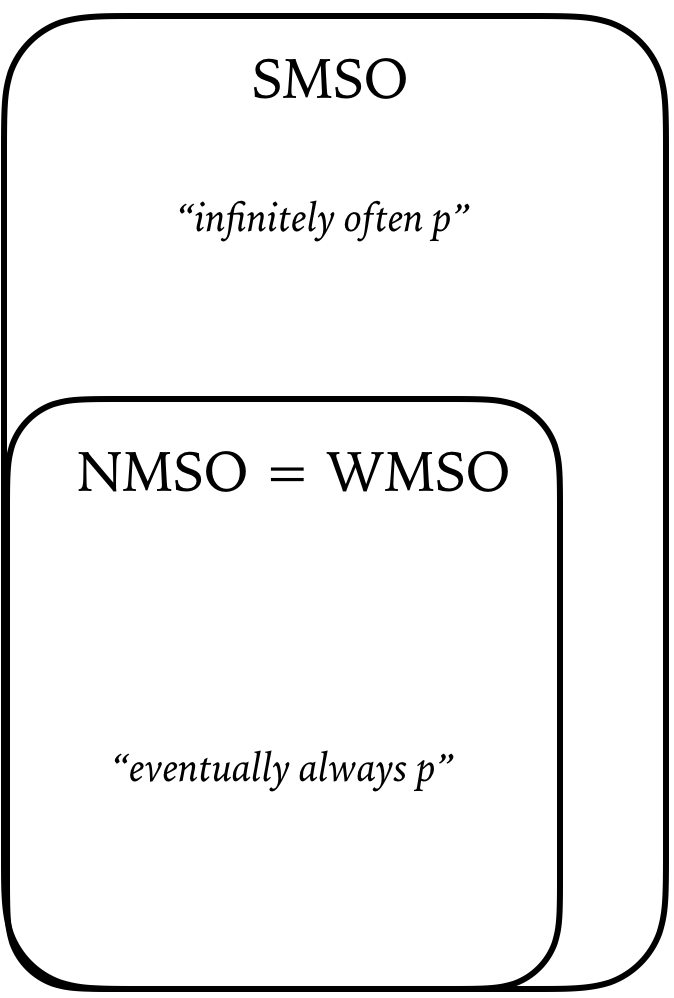
\includegraphics[width=\textwidth]{figures/fintree.png}
   \caption{On finitely branching trees}
   \label{fig:fintree}
\end{subfigure}
\begin{subfigure}[b]{0.3\textwidth}
    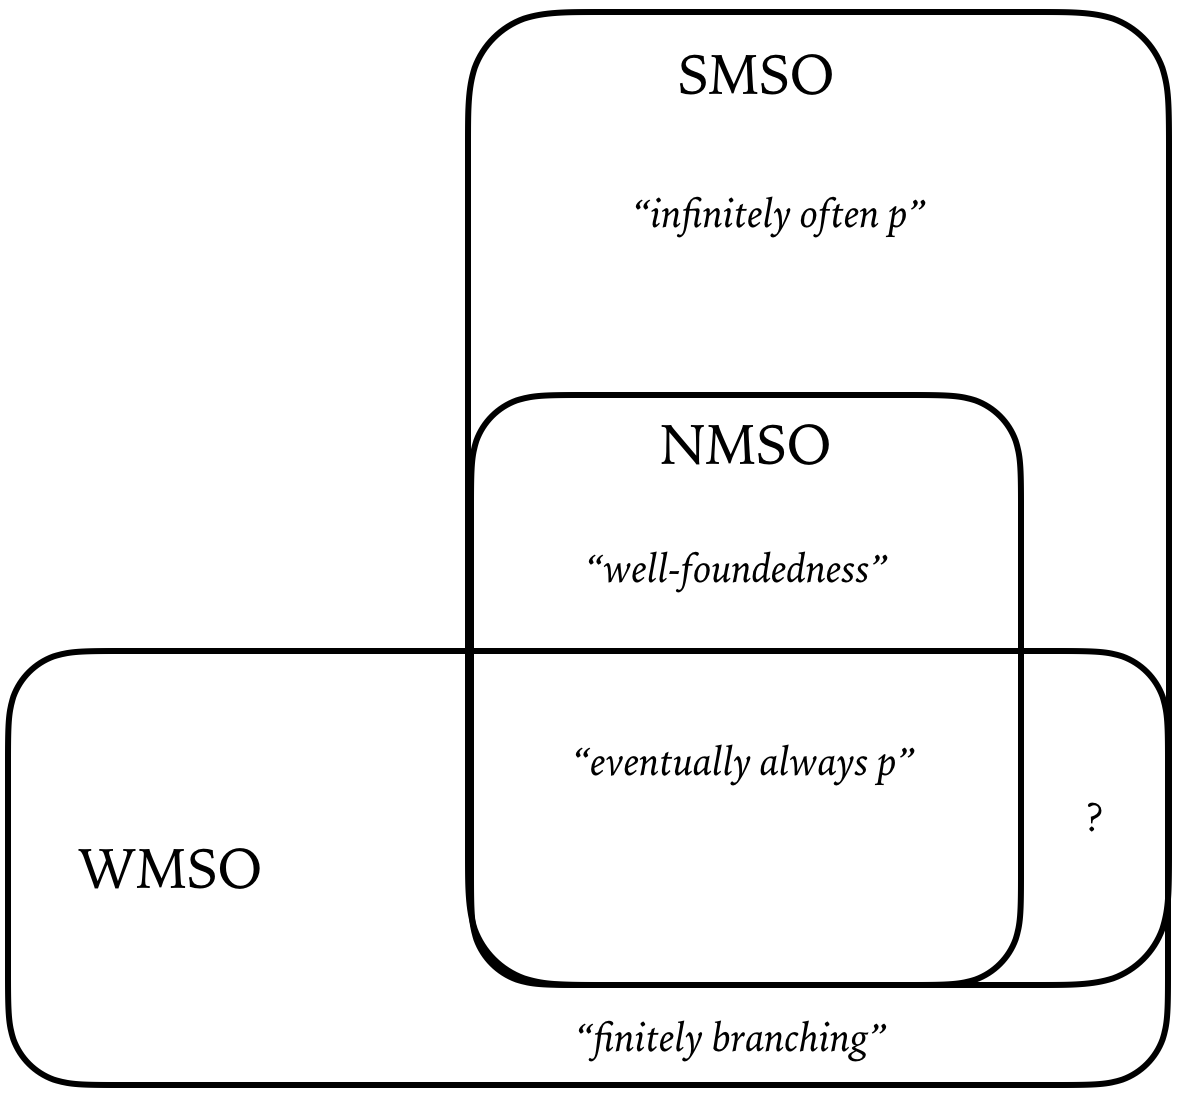
\includegraphics[width=\textwidth]{figures/tree.png}
    \caption{On arbitrary trees}
    \label{fig:tree}
\end{subfigure}
\begin{subfigure}[b]{0.3\textwidth}
    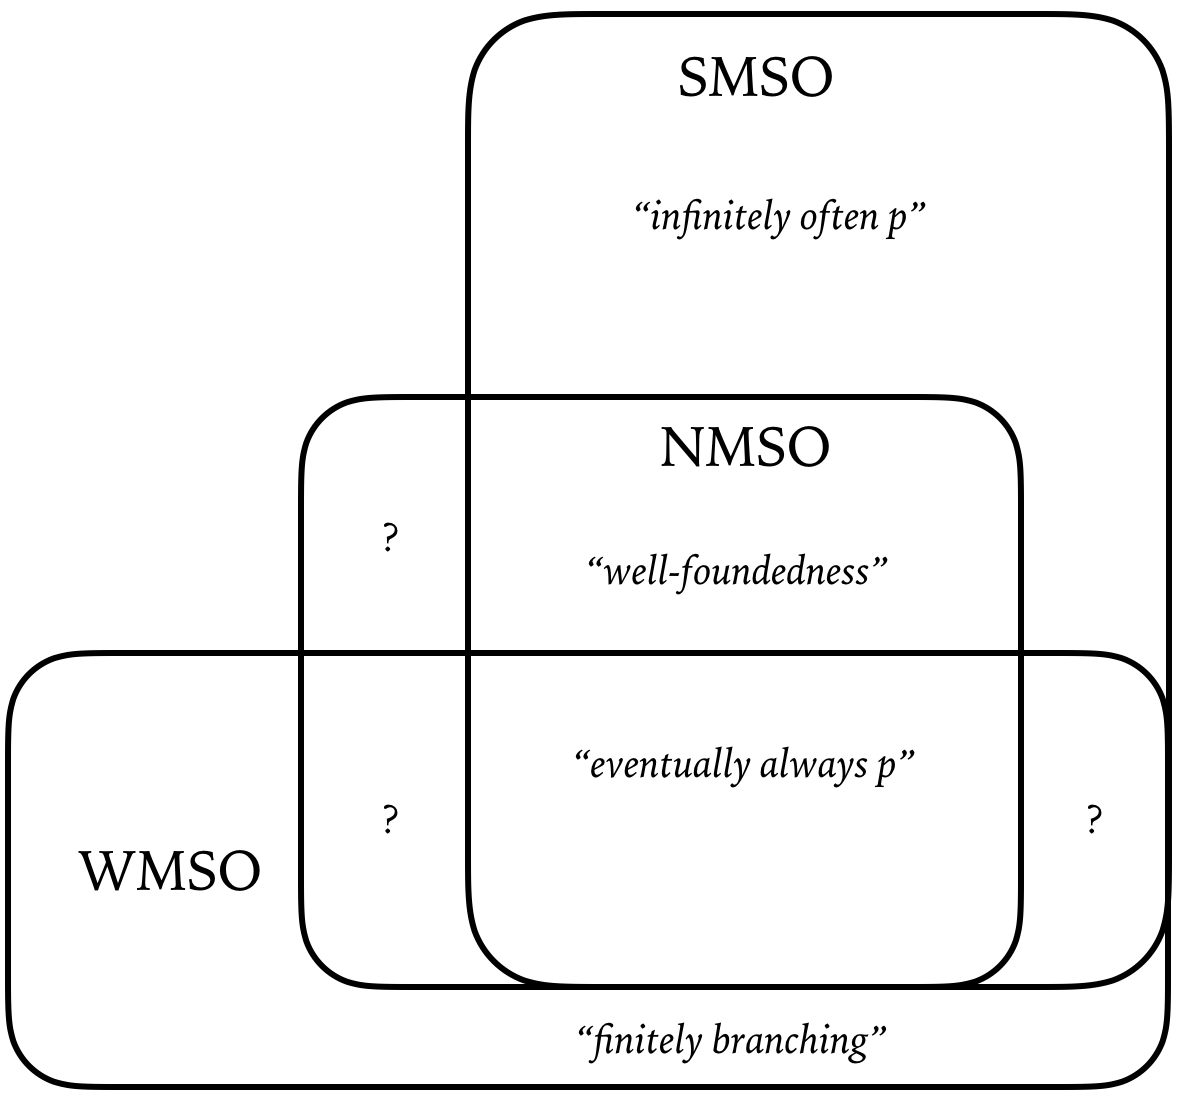
\includegraphics[width=\textwidth]{figures/slog.png}
    \caption{On arbitrary models}
    \label{fig:mouse}
\end{subfigure}
\caption{Expressiveness of three monadic second order logics}
\label{fig:lands}
\end{figure}

\subsection{Some model-theoretic observations}

Before we turn to the precise syntactic definition of the two fragments of 
$\muML$ that correspond to the monadic second-order logics $\wmso$ and $\nmso$,
we briefly discuss the fundamental \emph{semantic} properties underlying these
definitions.
Note that such a connection underlies the framework of the modal $\mu$-calculus
itself: the syntactic proviso on the formation of fixpoint formulas $\mu q.\phi$ 
(viz., the requirement that all occurrences of $q$ in $\phi$ are positive), 
guarantees a semantic property (namely: monotonicity of the associated semantic 
map $\phi^{\bbS}_{q}$), which is needed to use the Knaster-Tarski theorem 
to interpret the formula $\mu q.\phi$.

The idea underlying the definition of the fragments $\mucML$ and $\AFMC$ is to
impose further conditions on the formation of fixpoint formulas $\eta q. \phi$,
to ensure that the semantic map $\phi^{\bbS}_{q}$ satisfies some additional 
properties to be introduced now.

\begin{definition}
\label{d:cont}
Let $F: \wp S \to \wp S$ be a map.
We say that $F$ is \emph{monotone} if $F(X) \sse F(Y)$ whenever $X \sse Y$, and 
\emph{continuous} if it is monotone and satisfies 
\begin{equation}
\label{eq:Sc}
F(X) = \bigcup \{ F(Y) \mid Y \sse X, Y \text{ finite} \}.
\end{equation}
In case $S$ is the domain of a tree model, we call $F$ \emph{noetherian-based}
if it is monotone and satisfies the following 
condition
\begin{equation}
F(X) = \bigcup \{ F(Y) \mid Y \sse X, Y \text{ noetherian} \}.
\end{equation}
\end{definition}

In words, $F$ is continuous if it is completely determined by its action on 
finite sets, and a similar perspective applies to noetherian-based maps.
The name ``continuity'' is explained by the fact that a map $F: \wp S \to \wp S$
satisfies \eqref{eq:Sc} iff $F$ is continuous with respect to the \emph{Scott 
topology} on the power set $\wp(S)$ of $S$.
Scott continuity stems from \emph{domain theory}~\cite{abra94:doma}, and plays a 
fundamental role in many branches of logic and theoretical computer science that
feature ordered structures.

What is of interest here is that we may apply the concepts of 
Definition~\ref{d:cont} to \emph{formulas}.
To see how this works out for fixpoint formulas, recall the definition of the 
semantic map $\phi^{\bbS}_{q}$ associated with a formula $\phi \in \muML$ and a 
proposition letter $q$.

\begin{definition}
Let $\phi \in \muML$, and $q$ be a propositional variable. 
We say that \emph{$\phi$ is monotone (respectively, continuous/noetherian) in
$q$} if for every transition system $\bbS$, the map $\phi^{\bbS}_{q}: \wp S 
\to \wp S$ is monotone (respectively, continuous/noetherian).
\end{definition}

In fact, as part of the \emph{model theory} of the modal $\mu$-calculus, these
semantic properties (and many more) can be given rather exact syntactic 
characterisations.

\begin{definition}
Given a set $\qprop$ of propositional variables, we define the fragment 
$\noe{\mu\ML}{\qprop}$ of \muML-formulas that are (syntactically) 
\emph{noetherian} in $\qprop$, by the following grammar:
\begin{equation*}
   \phi \isbnf  q
   \mid \psi
   \mid \phi \lor \phi
   \mid \phi \land \phi
     \mid \Diamond \phi
       \mid \Box \phi
   \mid \mu p.\phi'
\end{equation*}
where $q \in \qprop$, $\psi$ is a $\qprop$-free $\muML$-formula, and 
$\phi' \in \noe{\mu\ML}{\qprop\cup\{p\}}$. 
The \emph{co-noetherian} fragment $\conoe{\mu\ML}{Q}$ is defined dually by 
taking $\nu$ instead of $\mu$ and stating $\phi' \in 
\conoe{\mu\ML}{\qprop\cup\{p\}}$.

Similarly, we define the fragment of \muML \emph{continuous} in $\qprop$, 
denoted by $\cont{\muML}{\qprop}$, by induction in the following way
\begin{equation*}
   \phi \isbnf  q
   \mid \psi
   \mid \phi \lor \phi
   \mid \phi \land \phi
   \mid \Diamond \phi
   \mid \mu p.\phi'
\end{equation*}
%
where $q,p \in \qprop$, $\psi$ is a $\qprop$-free $\muML$-formula and 
$\phi' \in \cont{\muML}{\qprop\cup\{p\}}$.
The  \emph{co-continuous} fragment $\cocont{\mu\ML}{Q}$ is defined dually 
by taking $\nu$ instead of $\mu$, $\Box$ instead of $\Diamond$ 
and stating $\phi' \in \cocont{\muML}{\qprop\cup\{p\}}$. 
\end{definition}

\begin{fact}[\cite{dago:logi00,Fontaine08,FV12}]
\label{f:mt}
The following hold, for any $\muML$-formula formula $\phi$, and any proposition
letter $q$:

(1) $\phi$ is monotone in $q$ iff it is equivalent to a formula $\phi'$
 which is positive in $q$;

(2) $\phi$ is continuous in $q$ iff it is equivalent to a formula $\phi'$
  in the fragment $\cont{\muML}{q}$;

(3) $\phi$ is noetherian in $q$ iff it is equivalent to a formula $\phi'$
   in the fragment $\noe{\muML}{q}$.
\end{fact}

In passing we note that in each instance of Fact~\ref{f:mt}, a slightly stronger
result can be proved, to the effect that it is \emph{decidable} whether a given
$\mu$-calculus formula is monotone (resp., continuous/noetherian) in a given
proposition letter.

\subsection{Fragments of the modal $\mu$-calculus}

We are now ready for the definition of the fragments $\AFMC$ and 
$\mucML$.
Starting with the first, note that
formulas of the modal $\mu$-calculus may be classified according to their
\emph{alternation depth}, which roughly is given as the maximal length of
a chain of nested alternating least and greatest fixpoint operators~\cite{Niwinski86}.
The \emph{alternation-free fragment} of the modal $\mu$-calculus~($\AFMC$) is 
usually defined as the collection of $\muML$-formulas without nesting of least
and greatest fixpoint operators. 
It can also be given a more standard grammatical definition as the fragment of 
the full language where we restrict the application of the least fixpoint 
operator $\mu p$ to formulas that are (syntactically) noetherian in $p$ (and 
apply a dual condition to the greatest fixpoint operator).

\begin{definition}
The formulas of the \emph{alternation-free} $\mu$-calculus $\AFMC$ are defined 
by the following grammar:
\begin{equation*}
   \phi \isbnf  
      q \mid \neg q  
   \mid \phi\lor\phi \mid \phi\land\phi 
      \mid \Diamond \phi
       \mid \Box \phi
   \mid \mu p. \phi'    
   \mid \nu p. \phi'',
\end{equation*} 
where $p,q \in \Prop$, $\phi' \in \AFMC \cap \noe{\mu\ML}{p}$
and dually $\phi'' \in \AFMC \cap \conoe{\mu\ML}{p}$.
\end{definition}

It is then immediate to verify that the above definition indeed captures exactly
all formulas without alternation of least and greatest fixpoints.
One may prove that a formula $\phi \in \muML$ belongs to the fragment $\AFMC$ 
iff for all subformulas $\mu p.\psi_1$ and $\nu q.\psi_2$ it holds that $p$ is
not free in $\psi_2$ and $q$ is not free in $\psi_1$.

Similarly, we define $\mucML$ to be the fragment of $\muML$ where the use of the
least fixed point operator is restricted to the continuous fragment. 

\begin{definition}
Formulas of the fragment $\mucML$ are given by:% the following induction:
\begin{equation*}
   \phi \isbnf  q \mid \lnot q
    \mid \phi \lor \phi
        \mid \phi \land \phi
    \mid \Diamond \phi
     \mid \Box \phi \mid
    \mu p.\phi' 
    \mid \nu p.\phi''
    \end{equation*}
%
where $p,q \in \Prop$,  $\phi' \in \cont{\muML}{p} \cap \mucML$, and dually 
$\phi'' \in \cocont{\muML}{p} \cap \mucML$.
\end{definition}

Characteristic about $\mucML$ is that in a formula $\mu p. \phi \in \mucML$, all
occurrences of $p$ in $\phi$ are \emph{existential} in the sense that they may 
be in the scope of a diamond but not of a box.
Furthermore, as an immediate consequence of Fact~\ref{f:mt}(2) we may make the 
following observation.

\begin{corollary}\label{cor:cont}
For every $\mucML$-formula $\mu p. \phi$, the formula $\phi$ is continuous in $p$.
\end{corollary}

% \btbs
% \item
% Over arbitrary transition systems, this fragment is less expressive than the 
% whole $\muML$~\cite{Park79}. 
% \etbs

Finally, we consider the relative expressiveness of the fixpoint languages
$\mucML$, $\AFMC$ and $\muML$.
It is immediate from the definitions that $\mucML \leq \AFMC \leq \muML$. 
Both inclusions are strict:
\begin{description}
\item[($\mucML \not\leq \AFMC$)] 
Consider the formula $\mu x. \Box x$ in $\AFMC$, stating that every path 
starting from the distinguished node of the model is finite. 
As mentioned already, on tree models this formula captures the property of being
conversely well-founded, which is known not be expressible in 
$\wmso$~\cite{CateF11}, and
hence, since $\mucML \leq \wmso$, not in the continuous 
$\mu$-calculus either.
\item[($\AFMC \not\leq \muML$)] 
The property ``on some path, $p$ holds infinitely often'' is definable by the
$\muML$-formula $\phi:=\nu x. \mu y. (( p \lor \Diamond y) \land \Diamond x)$.
However, this property is not definable in the alternation free fragment $\AFMC$.
This is because, for instance, on trees, every property definable in $\AFMC$ is 
also recognised by a B\"uchi-automata (see e.g. \cite{KupfermanVardi03}), 
whereas  ``infinitely often $p$'' is not \cite{Rab70}.  
\end{description}

\begin{remark}
\label{r:evalwp}
The discussion above, concerning the property ``on some path, $p$ holds 
infinitely  often'' may be contrasted with the rather similar-looking formula 
$\psi \isdef \mu x. \nu y. ( \Diamond x \lor (\Diamond y \land p))$. 
This formula states that there is a path in which from a certain point on $p$ 
always holds (``eventually always $p$''). 
Syntactically, $\psi$ is neither in $\AFMC$ (it has one alternation of 
fixpoints), nor a fortiori in $\mucML$. 
However, it is not difficult to see that $\psi$ is equivalent to the formula
$\mu x. \big( \Diamond x \lor \nu y \, (\Diamond y \land p)\big)$, which does
belong to the continuous $\mu$-calculus, and is in particular alternation free.
\end{remark}


